\section{Sphinx Packet Format}
\label{sec:sphinx}

HOPR uses the Sphinx packet format \cite{sphinxpaper} to encapsulate and route data packets in order to ensure sender and recipient unlinkability. The Sphinx packet format determines how mixnet packets are created and transformed before relaying them to the next downstream node in a way that does not leak path information to relayers or other parties. Each Sphinx packet consists of two parts, a header and an onion-encrypted payload:

\begin{figure}[H]
    \centering
    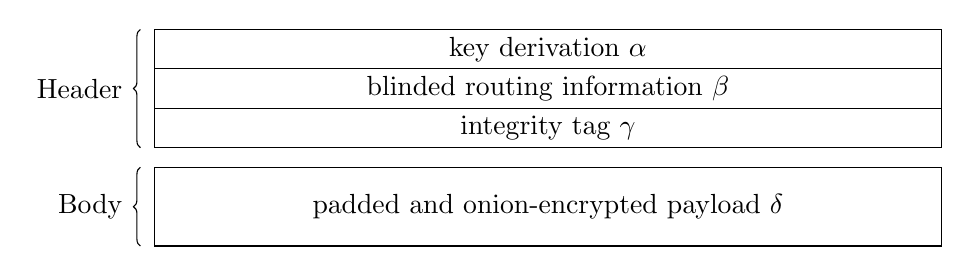
\begin{tikzpicture}
        \draw (0,0) rectangle (10,0.5);
        \draw (0,-0.5) rectangle (10,0);
        \draw (0,-1) rectangle (10,-0.5);

        \draw (5,0.25) node {key derivation $\alpha$};
        \draw (5,-0.25) node {blinded routing information $\beta$};
        \draw (5,-0.75) node {integrity tag $\gamma$};

        \draw[decoration={brace,raise=5pt,mirror},decorate] (0,0.5) -- node[left=8pt] {Header} (0,-1);

        \draw (0,-2.25) rectangle (10, -1.25);
        \draw (5,-1.75) node {padded and onion-encrypted payload  $\delta$};

        \draw[decoration={brace,raise=5pt,mirror},decorate] (0,-1.25) -- node[left=8pt] {Body} (0,-2.25);
    \end{tikzpicture}
    \label{fig:sphinxoverview}
    \caption{Schematic overview of a SPHINX packet}
\end{figure}

\subsection{Construction}

The following explains how a Sphinx packet is created and how it is transformed at each hop before arriving at its final destination. At first, the sender chooses a path (see Section \ref{sec:path-selection}), and derives shared keys with each node on the path. The shared keys serve as a master secret to derive subkeys. These subkeys are used to blind the routing information in such a way that nodes can solely determine the next downstream node, and also to create an authentication tag to check the integrity of the header. In addition, the sender applies one layer of encryption for each node along the chosen path to the payload. This accomplished, the sender finally sends the packet to the first hop.

Once a node receives a mixnet packet, it first derives the key that it has shared with the sender of the packet and checks the integrity of the header. Next, it unblinds the routing information to determine the next downstream node and removes one layer of encryption from the encrypted payload. At this point, the node is able to decide whether it is the final recipient of the message or it is supposed to forward the packet to the next hop.

\begin{comment}
\paragraph{Notation:}Let $\kappa=128$ be the security parameter. With non-negligible probability, an adversary must perform around $2^\kappa$ operations to break the security of Sphinx.

Let $r$ be the maximum number of nodes that a Sphinx mix message will traverse before being delivered to its destination.

$G$ is a prime order cyclic group satisfying the decisional Diffie-Hellman assumption \cite{Boneh_1998}. We use the secp256k1 elliptic curve \cite{secp}. The element $g$ is a generator of $G$ and $q$ is the (prime) order of $G$, with $q\approx2^{2*\kappa}$.

$G^*$ is the set of non-identity elements of G. $h_b$ is a pre-image resistant hash function used to compute blinding factors and modelled as a random oracle such that
$h_b:G^*\times G^*\rightarrow\mathbb{Z}^*_q$, where $\mathbb{Z}^*_q$ is the field of non-identity elements of $\mathbb{Z}_q$ (field of integers). We use the BLAKE2s hash function \cite{blake2}.

Each node $i$ has a private key $x_{i}\in \mathbb{Z}^*_q$ and a public key $y_{i}=g^{x_{i}}\in G^*$.
$\alpha_i$ is the group elements which, when combined with the nodes’ public keys, allow a shared key to be computed for each via Diffie-Hellman (DH) key exchange. This ensures that each node in the user-chosen route can forward the packet to the next, and only the receiving mix node can decrypt it.
$s_i$ are the DH shared secrets, $b_i$ are the blinding factors.
\end{comment}

\subsubsection{Key derivation}
\label{sec:sphinx:keyderivation}

The sender $A$ picks a random $x\in \mathbb{Z}^*_q$ that is used to derive new keys for every packet.

$A$ randomly picks a path consisting of intermediate nodes $B$, $C$, $D$, and the packet's final destination, $Z$.

$A$ performs an offline DH key exchange with each of these nodes and derives shared keys with each of them.

$A$ computes a sequence of $r$ tuples (in our case $r$=4)  $$(\alpha_0,s_0,b_0),.................,(\alpha_{r-1},s_{r-1},b_{r-1})$$ as follows:
$$\alpha_0=g^x,s_0=y^x_B,b_0=h_b(a_0,s_0)$$
and
\begin{equation}
    \begin{cases}
        \alpha_i=g^{x\Pi_{j=0}^{j=i-2}b_j} \\
        s_i=y^{x\Pi_{j=0}^{j=i-2}b_j}      \\
        b_i=h_b(a_i,s_i)
    \end{cases}\,.
    \label{eq:1}
\end{equation}
for $1\le i < r-1$, where $y_0,y_1, y_2, y_3$, and $y_4$ are the public keys of the nodes $B$, $C$, $D$, and $Z$, which we assume to be available to $A$ .
\subsubsection{Routing information}
\label{sec:sphinx:routinginformation}

Each node on the path needs to decide whether it is destined to be the receiver of the message and if not, to whom it is supposed to forward the packet. To achieve the privacy properties, each node must only know its direct predecessor and successor along the chosen path. More precisely, the node must not be able to determine \textit{if} and \textit{where} the next downstream node is going to forward the packet to. This is achieved by blinding that information such that it is visible to only that node who needs it.

To ensure that the header has not been tampered while transfered through the network and processed by nodes along the path, routing information contains also an integrity tag to check for modifications before processing the packet. Hence, the routing information for each node by $(y_i, \gamma_i)$ where $y_i$ denotes the public key and $\gamma_i$ the integrity tag for the next downstream node. See section \ref{sec:sphinx:integrity} for more details on the utilized integrity scheme.

\paragraph{Adresses}

Nodes in the network are distinguished by the ECDSA public keys, hence the header includes the public key of the next downstream node and a distinguished byte sequence $END$ to notify the last node on the path that it is the final recipient.

ECDSA public keys are given by tuple of two 32-byte field elements $(x,y)$, upon which it is sufficient to solely store the first component $x$ and the sign of $y$, resulting in a \textsf{compressed} elliptic curve point \textsf{0x02}\textless\textsf{x}\textgreater for positive $y$ and \textsf{0x03}\textless\textsf{x}\textgreater. The sequence $END$ is given as \textsf{0x04} such that the last node can ignore all subsequent bytes if $END$ is present.

\paragraph{Blinding}

The header uses multiple blindings and their aggregations to make certain sections of the header visible to only a single node. Blindings are generated by a pseudorandomness generator (PRG), see appendix \ref{appendix:prg} for a detailed description of the utilized PRG.

As a result of the Diffie-Helman key exchange done in section \ref{appendix:keyderivation}, each node along the path is able to derive a shared secret $s_i$ with the creator of the packet and is therefore able to derive a sub-key $s_i^{bl}$. Both, creator of the packet and each node $n_i$ along the path use $s_i^{bl}$ as a seed for the PRG, yielding $blinding_i$.

The routing information for each node $n_i$ is blinded by XORing the content with $blinding_i$ as well as the blindings $blinding_0, \dots , blinding_{i-1}$ of all previous hops. Each node that receives the packet, removes their own blinding from the header and is thus able extract the routing information destined for them. By removing the blinding from the header, it allows the next downstream node to extract their routing information since it is now only blinded by their blinding.

\begin{figure}[H]
    \centering
    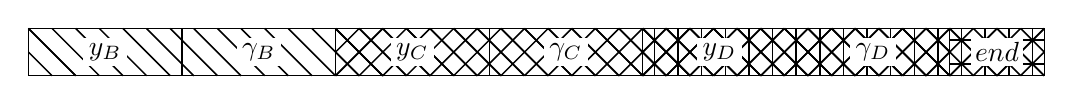
\begin{tikzpicture}
        \def\one{0.6}
        \def\scale{0.9}
        \def\nodeWidth{1.95}
        \def\endWidth{1.2}
        \def\width{3*2*\nodeWidth+\endWidth}
        \foreach \i\name in{0/B,1/C,2/D,3/Z} {
                \begin{scope}[shift={(\i*\nodeWidth*2,0)}]
                    \ifnum\i=0
                        \def\a{11.7}
                        \def\diff{11.1}
                    \fi

                    \ifnum\i=1
                        \def\a{7.8}
                        \def\diff{7.2}
                    \fi

                    \ifnum\i=2
                        \def\a{3.9}
                        \def\diff{3.3}

                    \fi

                    \ifnum\i=3
                        \def\a{\endWidth}
                        \def\diff{0.6}
                    \fi


                    \def\b{0.6}
                    \def\lw{0.2}

                    \foreach \x [count=\i] in{0,0.3,0.6,...,\b}{
                            \draw [line width=\lw mm](\x,0)--(0,\x) (\a-\b+\x,\b)--(\a,\x);
                        }
                    \foreach \x [count=\i] in{0,0.3,0.6,...,\diff}{
                            \draw [line width=\lw mm](\x+\b,0)--(\x,\b);
                        }

                    \ifnum\i>0
                        \foreach \x [count=\i] in{0,0.3,0.6,...,\b}{
                                \draw [line width=\lw mm](0,\x)--(\b-\x,\b) (\a-\b+\x,0)--(\a,\b-\x);
                            }
                        \foreach \x [count=\i] in{0,0.3,0.6,...,\diff}{
                                \draw [line width=\lw mm](\x,0)--(\b+\x,\b);
                            }
                    \fi

                    \ifnum\i>1
                        \foreach \x [count=\i] in{0.15,0.45,...,\a}{
                                \draw [line width=\lw mm](\x,0)--(\x,\b);
                            }
                    \fi

                    \ifnum\i>2
                        \foreach \x [count=\i] in{0.15,0.45,...,\b}{
                                \draw [line width=\lw mm](0,\x)--(\a,\x);
                            }
                    \fi
                \end{scope}
                \ifnum\i<3
                    \draw [color=white] (\i*2*\nodeWidth,0) rectangle (\i*2*\nodeWidth+\nodeWidth,\one) node [midway,color=black,fill=white,inner sep=2pt] {$y_{\name}$};
                    \draw (\i*2*\nodeWidth,0) -- (\i*2*\nodeWidth,\one);
                    \draw [color=white] (\i*2*\nodeWidth+\nodeWidth,0) rectangle (\i*2*\nodeWidth+2*\nodeWidth,\one) node [midway,color=black,fill=white,inner sep=2pt] {$\gamma_{\name}$};
                    \draw (\i*2*\nodeWidth+\nodeWidth,0) -- (\i*2*\nodeWidth+\nodeWidth,\one);
                \else
                    \draw [color=white] (\i*2*\nodeWidth,0) rectangle (\i*2*\nodeWidth+\endWidth,\one) node [midway,color=black,fill=white,inner sep=1.5pt] {$end$};
                    \draw (\i*2*\nodeWidth,0) -- (\i*2*\nodeWidth,\one);
                \fi
            }

        \draw (0,0) rectangle (\width,\one);
    \end{tikzpicture}
    \caption{Blinded routing information sent to first relayer $B$.}
\end{figure}

\paragraph{Filler}



such that $y_Z$ is the destination's public key in compressed form (since this is only the $x$-coordinate, it is 33 bytes instead of 64) and $|y_Z|$ is its length. $\rho$ is a pseudorandom generator (PRG) and $h_{\rho}$ is the hash function used to key $\rho$.
$v\leq r$ is the length of the path traversed by the packet, where $|y_Z| \leq (2(r - v) + 2)$. $\phi$ is a filler string such that
\begin{align}
    \phi_i & =\{ \phi_{i-1}\|0_{2\kappa}\}\oplus \rho(h_{\rho}(s_{i-1}))_{[ \,(2(r-i)+3)\kappa..(2r+3)\kappa-1\,]}
\end{align}
where $\phi_0=\epsilon$ is an empty string. $\phi_i$ is generated using the shared secret $s_{i-1}$ and used to ensure the header packets remain constant in size as layers of encryption are added or removed. Upon receiving a packet, the processing node extracts the information destined for it from the route information and the per-hop payload. The extraction is performed by deobfuscating and left-shifting the field. Ordinarily, this would make the field shorter at each hop, allowing an attacker to deduce the route length. For this reason, the field is pre-padded before forwarding. Since the padding is part of the HMAC, the origin node will have to pre-generate an identical padding (to that generated at each hop) in order to compute the HMACs correctly for each hop.

\begin{figure}[H]
    \centering
    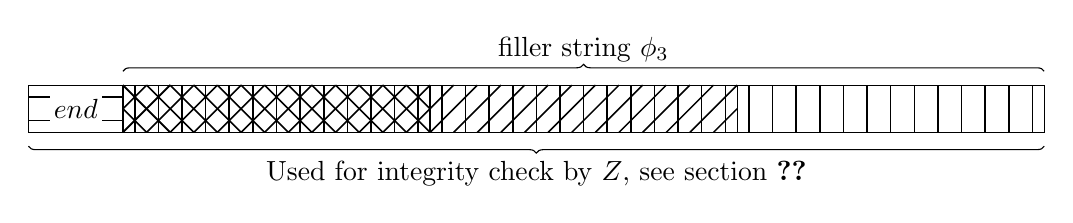
\begin{tikzpicture}
        \def\one{0.6}
        \def\scale{0.9}
        \def\nodeWidth{1.95}
        \def\endWidth{1.2}
        \def\width{3*2*\nodeWidth+\endWidth}
        \foreach \i\name in{0/B,1/C,2/D,3/Z} {
                \ifnum\i=3
                    \def\a{11.7}
                    \def\diff{11.1}
                \fi

                \ifnum\i=2
                    \def\a{7.8}
                    \def\diff{7.2}
                \fi

                \ifnum\i=1
                    \def\a{3.9}
                    \def\diff{3.3}

                \fi

                \ifnum\i=0
                    \def\a{\endWidth}
                    \def\diff{0.6}
                \fi


                \def\b{0.6}
                \def\lw{0.2}

                \begin{scope}[shift={(\endWidth,0)}]
                    \ifnum\i=1
                        \foreach \x [count=\i] in{0,0.3,0.6,...,\b}{
                                \draw [line width=\lw mm](\x,0)--(0,\x) (\a-\b+\x,\b)--(\a,\x);
                            }
                        \foreach \x [count=\i] in{0,0.3,0.6,...,\diff}{
                                \draw [line width=\lw mm](\x+\b,0)--(\x,\b);
                            }
                    \fi

                    \ifnum\i=2
                        \foreach \x [count=\i] in{0,0.3,0.6,...,\b}{
                                \draw [line width=\lw mm](0,\x)--(\b-\x,\b) (\a-\b+\x,0)--(\a,\b-\x);
                            }
                        \foreach \x [count=\i] in{0,0.3,0.6,...,\diff}{
                                \draw [line width=\lw mm](\x,0)--(\b+\x,\b);
                            }
                    \fi

                    \ifnum\i=3
                        \foreach \x [count=\i] in{0.15,0.45,...,\a}{
                                \draw [line width=\lw mm](\x,0)--(\x,\b);
                            }
                    \fi
                \end{scope}

                \ifnum\i=0
                    \foreach \x [count=\i] in{0.15,0.45,...,\b}{
                            \draw [line width=\lw mm](0,\x)--(\a,\x);
                        }
                \fi
                \ifnum\i>0
                    % \draw [color=white] (\i*2*\nodeWidth,0) rectangle (\i*2*\nodeWidth+\nodeWidth,\one) node [midway,color=black,fill=white,inner sep=2pt] {$y_{\name}$};
                    \draw (\i*2*\nodeWidth+\endWidth,0) -- (\i*2*\nodeWidth+\endWidth,\one);
                    % \draw [color=white] (\i*2*\nodeWidth+\nodeWidth,0) rectangle (\i*2*\nodeWidth+2*\nodeWidth,\one) node [midway,color=black,fill=white,inner sep=2pt] {$\gamma_{\name}$};
                    % \draw (\i*2*\nodeWidth+\nodeWidth,0) -- (\i*2*\nodeWidth+\nodeWidth,\one);
                \else
                    \draw [color=white] (\i*2*\nodeWidth,0) rectangle (\i*2*\nodeWidth+\endWidth,\one) node [midway,color=black,fill=white,inner sep=1.5pt] {$end$};
                    \draw (\endWidth,0) -- (\endWidth,\one);
                \fi
            }

        \draw (0,0) rectangle (\width,\one);
        \draw[decoration={brace,raise=5pt},decorate] (\endWidth,\one) -- node[above=5pt] {filler string $\phi_3$} (\width,\one);
        \draw[decoration={brace,mirror,raise=5pt},decorate] (0,0) -- node[below=7pt] {Used for integrity check by $Z$, see section \ref{sec:sphinx:integrity}} (\width,0);


    \end{tikzpicture}
    \caption{Transformed header as seen by $Z$}
\end{figure}

$\beta_i$ is computed as the concatenation of $y_Z$ and a sequence of padding which is then encrypted by XORing with the output of a PRG seeded with shared key $s_{v-1}$ of node $v-1$. The result is finally concatenated with $\phi$ to ensure the header packets remain constant in size.

In the original Sphinx paper, $y_Z$ is concatenated with an identifier $I$ and $0$ padding sequence, where $I$ is used for SURBs (single-use reply blocks) such that $I \in \{0, 1\}^\kappa$. We do not use $I$ since HOPR does not currently employ SURBs. We do, however, include $hint$ and $challenge$ values in $\beta$, defined in the \lcnameref{sec:proofofrelay} section. These values are not included in the original Sphinx paper but are needed for the HOPR protocol. Since $A$ has a shared secret with each of the nodes along the path, it is able to derive blindings for each of them. Each node along the path receives an authentication tag $\gamma_i$ in the form of a message authentication code (MAC), which is encoded in the header.

Padding is added at each mix stage in order to keep the length of the message invariant at each hop.

The mix header is constructed as follows:
\begin{align}
    M_i & =(\alpha_i,\beta_i,\gamma_i)
\end{align}

$A$ sends the mix header $M_0$ to $B$. Once $B$ receives the packet, it derives the shared key $s_0$ by computing

$$s_0=(\alpha_0)^b=(g^x)^b=(g^b)^x=y^x_B$$

and removes its blindings. Here $b$ is the private key of node B. This allows $B$ to unblind the routing info that tells $B$ the public key of the next downstream node, $C$. The process happens in the same fashion for all further downstream nodes after $B$.


\subsubsection{Integrity check}
\label{sec:sphinx:integrity}

The integrity check allows the node to verify whether or not the header has been modified. By using the derived shared secret $s_i$, each node is able to recompute the authentication tag and check the integrity of the received packet as follows:
\begin{align}
    \gamma_i & =HMAC(s_i,\beta_i)
    \label{eq:6}
\end{align}
$B$ computes the keyed hash of the encrypted routing information $\beta_0$ as

$$\gamma_0=HMAC(s_0,\beta_0)$$
and compares with the integrity tag $\gamma_0$ attached in the packet header. If the integrity check fails, it is assumed the header has been tampered with and the packet is dropped. Otherwise, the mix node proceeds to the unblinding step. The HOPR packet header contains one integrity tag $\gamma_i$ for each node along the path.
\subsubsection{Unblinding}
\label{sec:sphinx:unblinding}

The unblinding works as follows: $B$ decrypts the attached $\beta_0$ in order to extract the routing instructions. First, $B$ appends a zero-byte padding at the end of $\beta_0$ and decrypts the padded block of routing information $\beta$ by XORing it with $PRG(s_{0})$ as follows:
\begin{align}
    (\beta_0\|0_{2\kappa}) & \oplus \rho(h_{\rho}(s_{0}))
\end{align}
$B$ parses the routing instructions from $A$ in order to obtain the address of the next mix node, $C$, as well the new integrity tags $\gamma_1$ and $\beta_1$, which should be forwarded to the next hop.
\subsubsection{Delete and shift}
\label{sec:sphinx:shifting}

After $B$ extracts the public key of $C$, it deletes the routing information from the packet. $B$ then fills the empty space with its own blinding (which is different from the one received from $A$) by setting the key share $\alpha_0$ to $\alpha_1=g^{xb_0}$. $B$ also computes $\beta_1$ as follows:

The first $\kappa$ bits of $\beta_0$ will be $n_{1}$ itself, the next $\kappa$ bits will be $\gamma_{1}$, and the remaining $(2r-1)\kappa$ bits of $\beta_0$ are shifted left to form the leftmost $(2r-1)\kappa$ bits of $\beta_{1}$; the rightmost $2\kappa$ bits of $\beta_{1}$ are simply a substring of an output of the PRG function.

\begin{figure}[H]
    \centering
    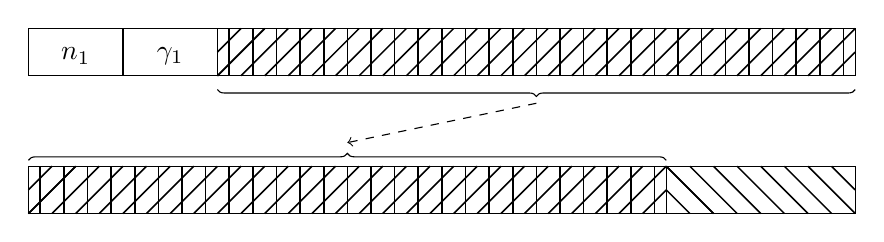
\begin{tikzpicture}
        \def\betaLength{10.5}
        \def\pubKey{1.2}
        \def\authTag{1.2}
        \draw (0,0) rectangle (\betaLength,0.6);

        \draw (0.6, 0.25) node {$n_1$};
        \draw (1.8, 0.25) node {$\gamma_1$};

        \draw (\pubKey,0) -- (\pubKey,0.6) (\pubKey+\authTag,0) -- (\pubKey+\authTag,0.6);

        \draw[decoration={brace,raise=5pt,mirror},decorate] (\authTag+\pubKey,0) -- (\betaLength,0);

        \def\halfBeta{{(\betaLength-\pubKey-\authTag)}*0.5}
        \draw [->,dashed] (4.05+\pubKey+\authTag, -0.35) -- (4.05, -0.85);

        \draw[decoration={brace,raise=5pt},decorate] (0,-1.25) -- (\betaLength-\authTag-\pubKey,-1.25);

        \begin{scope}[shift={(\pubKey+\authTag,0)}]
            \def\a{8.1}
            \def\b{0.6}
            \def\lw{0.2}
            \def\diff{7.5}

            \foreach \x [count=\i] in{0,0.3,0.6,...,\b}{
                    \draw [line width=\lw mm](0,\x)--(\b-\x,\b) (\a-\b+\x,0)--(\a,\b-\x);
                }
            \foreach \x [count=\i] in{0,0.3,0.6,...,\diff}{
                    \draw [line width=\lw mm](\x,0)--(\b+\x,\b);
                }

            \foreach \x [count=\i] in{0,0.15,0.45,...,\a}{
                    \draw [line width=\lw mm](\x,0)--(\x,\b);
                }
        \end{scope}

        \begin{scope}[shift={(0, -1.75)}]
            \draw (0,0) rectangle (\betaLength,0.6);
            \draw (\betaLength-\pubKey-\authTag, 0) -- (\betaLength-\pubKey-\authTag, 0.6);

            \begin{scope}[shift={(0,0)}]
                \def\a{8.1}
                \def\b{0.6}
                \def\lw{0.2}
                \def\diff{7.5}

                \foreach \x [count=\i] in{0,0.3,0.6,...,\b}{
                        \draw [line width=\lw mm](0,\x)--(\b-\x,\b) (\a-\b+\x,0)--(\a,\b-\x);
                    }
                \foreach \x [count=\i] in{0,0.3,0.6,...,\diff}{
                        \draw [line width=\lw mm](\x,0)--(\b+\x,\b);
                    }

                \foreach \x [count=\i] in{0,0.15,0.45,...,\a}{
                        \draw [line width=\lw mm](\x,0)--(\x,\b);
                    }
            \end{scope}

            \begin{scope}[shift={(\betaLength-\pubKey-\authTag,0)}]
                \def\a{2.4}
                \def\b{0.6}
                \def\lw{0.2}
                \def\diff{1.8}
                \foreach \x [count=\i] in{0,0.3,0.6,...,\b}{
                        \draw [line width=\lw mm](\x,0)--(0,\x) (\a-\b+\x,\b)--(\a,\x);
                    }
                \foreach \x [count=\i] in{0,0.3,0.6,...,\diff}{
                        \draw [line width=\lw mm](\x+\b,0)--(\x,\b);
                    }
            \end{scope}
        \end{scope}

    \end{tikzpicture}
    \caption{Shifting in the header}
\end{figure}

The new mix header is now ready to be sent to $C$, defined as the node with public key $y_1$:

$$M_1=(\alpha_1,\beta_1,\gamma_1)$$

where $\alpha$, $\beta$ and $\gamma$ are defined in equations $\ref{eq:1}$, $\ref{eq:2}$ and $\ref{eq:6}$
\subsubsection{Encrypt and decrypt}
\label{sec:sphinx:payload}

In contrast to the header, the integrity of the payload is not directly protected by the protocol. To ensure potential manipulations of the message remain visible to the final recipient, the content of the payload is hidden using a pseudorandom permutation scheme (PRP) and its inverse is used to undo the transformation. This comes with the property that if there were any modifications to the payload, such as a bit flip, the probability that the decoded message contains any relevant information is expected to be negligible.

To implement the PRP, HOPR uses the LIONESS \cite{lionesspaper} wide-block cipher scheme, instantiated by using Chacha20 as a stream cipher and BLAKE2s as a hash function as suggested by \href{https://katzenpost.mixnetworks.org/docs/specs/lioness.html}{Katzenpost}. See appendix \ref{appendix:lioness} for a detailed description and the chosen parameters.

As seen in Section \ref{sec:sphinx:keyderivation}, while creating the packet the sender derives a shared key $s_i$ with each node along the chosen path and uses them to create subkeys $s_i^{prp}$ to key the PRP. See Appendix \ref{appendix:keyderivation} for more details about the key derivation.

To allow the final recipient to determine whether a message is meaningful content or not, each message is padded by a protocol-specific tag $\tau$ and 0s to fit the packet size of 500 bytes, yielding $m_{pad}$. Decoded payloads that do not include $\tau$ are considered invalid and should be dropped.

\begin{figure}[H]
    \centering
    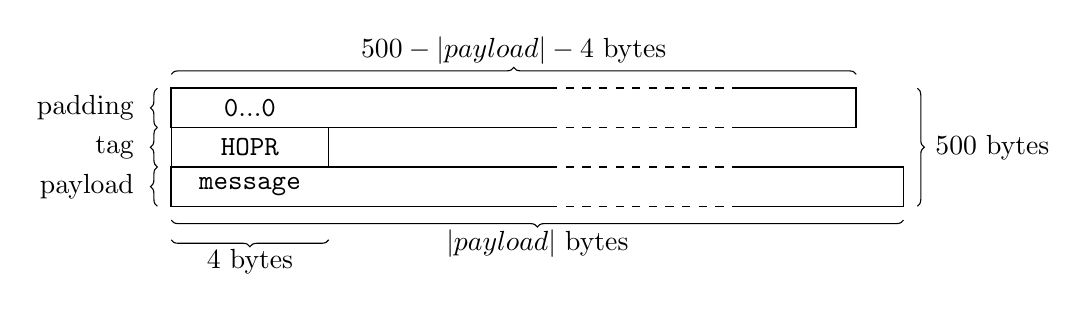
\begin{tikzpicture}
        \def\one{0.3}
        \def\lw{0.2}
        \def\middle{16*\one}
        \def\offset{8*\one}
        \def\packetLength{500}

        \def\paddingLength{29*\one}
        \def\payloadLength{31*\one}


        \draw[decoration={brace,raise=5pt},decorate] (0,0.5) -- node[above=5pt] {$\packetLength - |payload| - 4$ bytes} (\paddingLength,0.5);
        \begin{scope}
            \draw[decoration={brace,raise=5pt},decorate] (0,0) -- node[left=10pt] {padding} (0,0.5);
            \def\width{\paddingLength}
            \draw (1,0.25) node {$\mathtt{0...0}$};
            \draw [line width=\lw mm] (\middle,0.5) -- (0,0.5) --  (0,0) -- (\middle,0);
            \draw [line width=\lw mm] (\middle,0) --  (\middle+\offset, 0) [dashed];
            \draw [line width=\lw mm] (\middle,0.5) --  (\middle+\offset, 0.5) [dashed];
            \draw [line width=\lw mm] (\middle+\offset,0.5) -- (\width,0.5) --  (\width,0) -- (\middle+\offset,0);
        \end{scope}

        \begin{scope}[shift={(0,-0.5)}]
            \draw[decoration={brace,raise=5pt},decorate] (0,0) -- node[left=10pt] {tag} (0,0.5);
            \draw [draw] (0,0) rectangle (2,0.5);
            \draw (1,0.25) node {$\mathtt{HOPR}$};
        \end{scope}

        \begin{scope}[shift={(0,-1)}]
            \draw[decoration={brace,raise=5pt},decorate] (0,0) -- node[left=10pt] {payload} (0,0.5);
            \draw (1,0.25) node {$\mathtt{message}$};
            \def\width{\payloadLength}
            \draw [line width=\lw mm] (\middle,0.5) -- (0,0.5) --  (0,0) -- (\middle,0);
            \draw [line width=\lw mm] (\middle,0) --  (\middle+\offset, 0) [dashed];
            \draw [line width=\lw mm] (\middle,0.5) --  (\middle+\offset, 0.5) [dashed];
            \draw [line width=\lw mm] (\middle+\offset,0.5) -- (\width,0.5) --  (\width,0) -- (\middle+\offset,0);
        \end{scope}

        \draw[decoration={brace,raise=5pt,mirror},decorate] (0,-1.0) -- node[below=5pt] {$|payload|$ bytes} (\payloadLength,-1.0);
        \draw[decoration={brace,raise=5pt,mirror},decorate] (0,-1.25) -- node[below=5pt] {4 bytes} (2,-1.25);

        \draw[decoration={brace,raise=5pt},decorate] (\payloadLength,0.5) -- node[right=8pt] {$\packetLength$ bytes} (\payloadLength,-1.0);
    \end{tikzpicture}
    \caption{Padded message consisting of 0-padding, protocol tag $\tau$ ($\mathtt{0x484f5052}$, ASCII-encoded ``HOPR"), and payload $m$.}
\end{figure}

The sender takes the padded message and encrypts it using $\mathsf{PRP.permutate}$ with the derived subkeys in reverse order ($...,s_{i+1}^{prp}, s_i^{prp}, s_{i-1}^{prp},....$)

$$\delta_i = \mathsf{PRP.permutate}_{s_i^{prp}}(\delta_{i+1})$$

where $\delta_4 = m_{pad}$ and $\delta_0$ is the ciphertext that is sent to the first relayer when using three intermediate hops.

Each node $n_i$ along the chosen path then removes one layer of encryption by setting

$$\delta_{i-1} = \mathsf{PRP.inverse}_{s_i^{prp}}(\delta_i)$$

yielding $\delta_0 = m_{pad}$ in case the node is the final recipient.



\subsection{Implementation choices}

HOPR employs the following cryptographic primitives:

\begin{itemize}
    \item \textbf{Cyclic group} HOPR's Sphinx implementation uses an elliptic curve group on the secp256k1 curve. Operations are therefore performed on the elliptic curve.

    \item \textbf{Hash function} HOPR uses the BLAKE2s hash function, a cryptographic hash function faster than SHA-2 and SHA-3, yet at least as secure as SHA-3. It produces digests of 32 bytes.

    \item \textbf{MAC} HOPR uses HMAC based on the BLAKE2s hash function.

    \item \textbf{Encryption scheme} HOPR uses the LIONESS \cite{lionesspaper} implementation, using BLAKE2s as a hash function and ChaCha20 as a stream cipher.

    \item \textbf{Padding} The original Sphinx paper uses a sequence of 0s for padding. However, this allows the last mix node in the path to infer information about the length of the path and the final destination, hence breaking one of the security properties promised by Sphinx. In order to prevent this attack, HOPR replaces the 0-padding with randomized padding for the final mix node when $v<r$. This ensures the exit node cannot identify where the padding starts and thus will not be able to determine the path length. In the case where $v=r$ there is no need to add padding as the length of the path is the maximum length, and thus no additional information is being revealed.

\end{itemize}
